\documentclass{article}
\usepackage{amsmath}
\usepackage{mathtools}
\usepackage{gensymb}
\usepackage[a4paper,inner=1.5cm,outer=1.5cm,top=2cm,bottom=0.5cm]{geometry} 
\usepackage{xcolor}                    
\usepackage{tikz}                           
\usepackage{multicol}
\usepackage{pgfplots}
\usetikzlibrary{calc}
\usetikzlibrary{intersections}
\usetikzlibrary{intersections,calc,angles,quotes}
\usetikzlibrary{shapes,arrows,positioning,decorations.pathreplacing,calc}
\usetikzlibrary{calc,angles,positioning,intersections,quotes,decorations.markings}
\usepackage{tkz-euclide}
\usetikzlibrary{backgrounds}
\usetikzlibrary{calc,through}
\usetikzlibrary{angles}
\usetikzlibrary{fadings}
\usetikzlibrary{shapes.geometric}
\usetikzlibrary{shapes.symbols}
\usepackage{draftwatermark}
\usepackage{mathptmx}

\SetWatermarkText{\textcolor{black!30}{Mathema Shukur}}
\SetWatermarkFontSize{2 cm}
\usepackage[utf8]{inputenc}
\usepackage{fontspec}

\setmainfont{[Kalpurush.ttf]}
\newfontface{\en}{[Arial.ttf]} %%this is optional, if you want to use a secondary font. Any english font is supported
\newlength\Radius
\setlength\Radius{4cm}
\begin{document} 
	\Large
	\textcolor{red}{Welcome To} 
	\\
	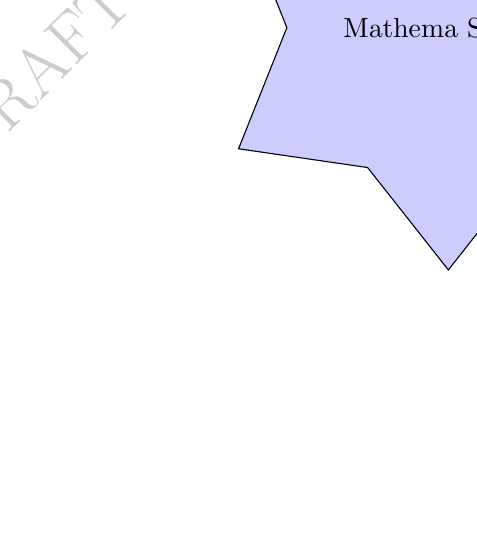
\begin{tikzpicture}
		\tikz \node [fill=blue!20,star,star points=6,draw] {Mathema Shukur };
	\end{tikzpicture}
	\\
	যাদের জন্যে প্রযোজ্যঃ  	\textcolor{magenta}{একাদশ ও দ্বাদশ শ্রেণীর শিক্ষার্থী} \\
	বিষয়ঃ \textcolor{magenta}{উচ্চতর গণিত ১ম পত্র} \\
	অধ্যায়ঃ \textcolor{magenta}{৩-সরলরেখা}\\ 
	Subtopicঃ  \textcolor{magenta}{ দুইটি বিন্দুর মধ্যবর্তী দূরত্ব নির্ণয় করা }\\
	\\
	$A(x_1,y_1)$ ও $B(x_2,y_2)$ বিন্দুর মধ্যবর্তী দূরত্ব $AB$\\
	\\ 
	\begin{tikzpicture}[transform shape,scale=1]
	\draw [-latex,thick](-2,0) -- (8,0) node[right] {$x$} coordinate(x axis);
	\draw [-latex,thick](0,-2) -- (0,8) node[above] {$y$} coordinate(y axis);
	\fill[black] (0,0) circle (1.5 mm);
	\node at (0.5,-0.5) {$\textcolor{purple}{(0,0)}$};
	\fill[red] (2,2) circle (1 mm);
	\fill[red] (7,7) circle (1 mm);
	\node at (4.5,1.5) {$\textcolor{red}{x_2-x_1}$};
	\node at (8,4.5) {$\textcolor{red}{y_2-y_1}$};
	\node at (1.7,2.5) {$\textcolor{red}{A}$};	
	\node at (7,7.5) {$\textcolor{red}{B}$};
	\node at (7.5,2) {$\textcolor{red}{C}$};	
	\node at (2,-0.5) {$\textcolor{blue}{x_1}$};		
	\node at (7,-0.5) {$\textcolor{blue}{x_2}$};		
	\node at (-0.5,2) {$\textcolor{blue}{y_1}$};		
	\node at (-0.5,7) {$\textcolor{blue}{y_2}$};					
	\draw[thick,red] (2,2)--(7,7);
	\draw[thick,dashed,blue] (0,2)--(2,2);
	\draw[thick,dashed,blue] (2,0)--(2,2);
	\draw[thick,dashed,blue] (0,7)--(7,7);
	\draw[thick,dashed,blue] (7,0)--(7,7);
	\draw[thick,dashed,red] (2,2)--(7,2);
\end{tikzpicture}
\\ 
$ABC$ সমকোণী ত্রিভুজে পীথাগোরাসের উপপাদ্য প্রয়োগ করে পাই \\
\begin{align*}
	AB^2&=AC^2+BC^2\\
	\\
	AB^2&=(x_2-x_1)^2+(y_2-y_1)^2\\
	\\
	AB&=\sqrt{(x_2-x_1)^2+(y_2-y_1)^2}
\end{align*}
\\ 
	দুইটি বিন্দু $(x_1,y_1)$ ও $(x_2,y_2)$এর মধ্যবর্তী দূরত্ব $d=\sqrt{(x_1-x_2)^2+(y_1-y_2)^2}$\\
	\\ 
	(চট্রগ্রাম বোর্ড-২০২১)\\
$(3,4)$ হতে $(-1,1)$ বিন্দুর দূরত্ব নির্ণয় কর \\
\\
$(x_1,y_1)=(3,4)$ ও $(x_2,y_2)=(-1,1)$এর মধ্যবর্তী দূরত্ব \\
\begin{align*}
	d&=\sqrt{(x_1-x_2)^2+(y_1-y_2)^2}\\
	\\
		d&=\sqrt{(3-(-1))^2+(4-1)^2}\\
		\\
		d&=\sqrt{(4)^2+(3)^2}\\
		\\
		d&=\sqrt{16+9}\\
		\\
		d&=\sqrt{25}\\
		\\
		d&=5
\end{align*}
\\ 
\includegraphics[width=5cm]{dis2points}
\\
(ঢাকা বোর্ড-২০২১)\\
$y$ অক্ষ ও $(2,2)$ বিন্দু থেকে $(a,5)$ বিন্দুটির দূরত্ব সমান হলে $a$ এর মান নির্ণয় কর \\ 
\\
	\begin{tikzpicture}[transform shape,scale=1]
	\draw [-latex,thick](-2,0) -- (6,0) node[right] {$x$} coordinate(x axis);
	\draw [-latex,thick](0,-2) -- (0,6) node[above] {$y$} coordinate(y axis);
	\fill[black] (0,0) circle (1.5 mm);
	\node at (0.5,-0.5) {$\textcolor{purple}{(0,0)}$};
	\fill[red] (2,2) circle (1 mm);
	\fill[red] (3,5) circle (1 mm);
	\node at (2.8,2) {$\textcolor{red}{(2,2)}$};			
	\draw[thick,dashed,blue] (2,2)--(3,5);
		\draw[thick,dashed,blue] (0,5)--(3,5);
			\node at (3.8,5) {$\textcolor{red}{(a,5)}$};
		\node at (1.5,5.3) {$\textcolor{blue}{a}$};		
\end{tikzpicture}
\\ 
$y$ অক্ষ  থেকে $(a,5)$ বিন্দুটির দূরত্ব =|বিন্দুটির ভুজ |=  $d_1=|a|$\\
\\ 
 $(2,2)$ বিন্দু থেকে $(a,5)$ বিন্দুটির দূরত্ব \\
 \\
 \begin{align*}
 	d_2&=\sqrt{(x_1-x_2)^2+(y_1-y_2)^2}\\
 	\\
 	d_2&=\sqrt{(2-a)^2+(2-5)^2}\\
 	\\
 	d_2&=\sqrt{2^2-2\,\,a\,\,2+a^2+(-3)^2}\\
 	\\
 	d_2&=\sqrt{4-4\,\,a+a^2+9}\\
 	\\
 	d_2&=\sqrt{a^2-4\,a+13}\\
 \end{align*}
\\ 
$y$ অক্ষ ও $(2,2)$ বিন্দু থেকে $(a,5)$ বিন্দুটির দূরত্ব সমান \\ 
\begin{align*}
	d_2&=d_1\\
	\\
	\sqrt{a^2-4\,a+13}&=|a|\\
	\\
	a^2-4\,a+13&=a^2\\
	\\
	-4\, a&=-13\\
	\\
	a&=\frac{13}{4}
\end{align*}
পোলার স্থানাঙ্কে  $(r_1,\theta_1)$ এবং  $(r_2,\theta_2)$ বিন্দুদ্বয়ের মধ্যবর্তী দূরত্ব  $d=\sqrt{r_1^2+r_2^2-2r_1\,\,r_2 \cos (\theta_1-\theta_2)}$\\
\\ 
শাহজালাল বিজ্ঞান ও প্রযুক্তি বিশ্ববিদ্যালয় ভর্তি পরীক্ষা- ২০১৯-২০২০\\
দুইটি বিন্দুর পোলার স্থানাঙ্ক $(2\sqrt{3},90\degree)$ এবং $(2\sqrt{5},180\degree)$ হলে  বিন্দু দুইটির দূরত্ব কত? \\ 
\\ 
$(r_1,\theta_1)=(2\sqrt{3},90\degree)$ এবং  $(r_2,\theta_2)=(2\sqrt{5},180\degree)$
\\
\begin{align*}
d&=\sqrt{r_1^2+r_2^2-2r_1\,\,r_2 \cos (\theta_1-\theta_2)}\\
\\
d&=\sqrt{(2\sqrt{3})^2+(2\sqrt{5})^2-2(2\sqrt{3})\,\,(2\sqrt{5})\cos (90\degree-180\degree)}\\
\\
d&=\sqrt{12+20-8\sqrt{15}\cos (-90\degree)}\\
\\
d&=\sqrt{12+20-8\sqrt{15}\,\,(0)}\\
\\
d&=\sqrt{32}\\
\\
d&=4\sqrt{2}
\end{align*}
\end{document}